%% fig_delsarte.tex   (generated by make_round21.py; do not edit by hand)
%% The 29 Delsarte sextic fourfolds built from Fermat terms, chains and loops (prop:delsarte), with the degree d of the least Fermat fourfold that covers each.
\documentclass[tikz,border=8pt]{standalone}
\usepackage{amsmath,amssymb}
\usetikzlibrary{arrows.meta,calc,decorations.pathreplacing}
%% palette.tex -- shared colour definitions for the figures
\definecolor{PInk}{RGB}{26,32,44}
\definecolor{PBlue}{RGB}{37,82,139}
\definecolor{PTeal}{RGB}{23,127,125}
\definecolor{POchre}{RGB}{193,138,44}
\definecolor{PClay}{RGB}{178,74,58}
\definecolor{PSlate}{RGB}{108,122,137}
\definecolor{PViolet}{RGB}{110,86,150}
\definecolor{WBlue}{RGB}{223,234,246}
\definecolor{WTeal}{RGB}{220,238,236}
\definecolor{WOchre}{RGB}{250,240,218}
\definecolor{WClay}{RGB}{247,229,224}
\definecolor{WSlate}{RGB}{238,241,244}
\definecolor{PMag}{RGB}{158,58,110}
\definecolor{PGrass}{RGB}{62,124,66}
\definecolor{PAmber}{RGB}{214,112,38}
\definecolor{PIndigo}{RGB}{58,64,140}
\definecolor{PRule}{RGB}{176,186,197}

%% shared macros so the standalone figures match the paper
\providecommand{\QQ}{\mathbb{Q}}
\providecommand{\ZZ}{\mathbb{Z}}
\providecommand{\RR}{\mathbb{R}}
\providecommand{\CC}{\mathbb{C}}
\providecommand{\PP}{\mathbb{P}}
\providecommand{\Kx}{K^{\times}}
\providecommand{\HW}{W}
\providecommand{\Nm}{\mathrm{N}}
\providecommand{\Hdg}{\mathrm{Hdg}}
\providecommand{\NS}{\mathrm{NS}}
\providecommand{\cA}{\mathcal{A}}
\providecommand{\cD}{\mathcal{D}}
\providecommand{\cF}{\mathcal{F}}
\providecommand{\cP}{\mathcal{P}}
\providecommand{\cO}{\mathcal{O}}
\providecommand{\cQ}{\mathcal{Q}}
\providecommand{\bbar}[1]{\overline{#1}}
\providecommand{\ch}{\operatorname{ch}}
\providecommand{\End}{\mathrm{End}}
\providecommand{\Ext}{\operatorname{Ext}}
\providecommand{\Supp}{\operatorname{Supp}}

\begin{document}
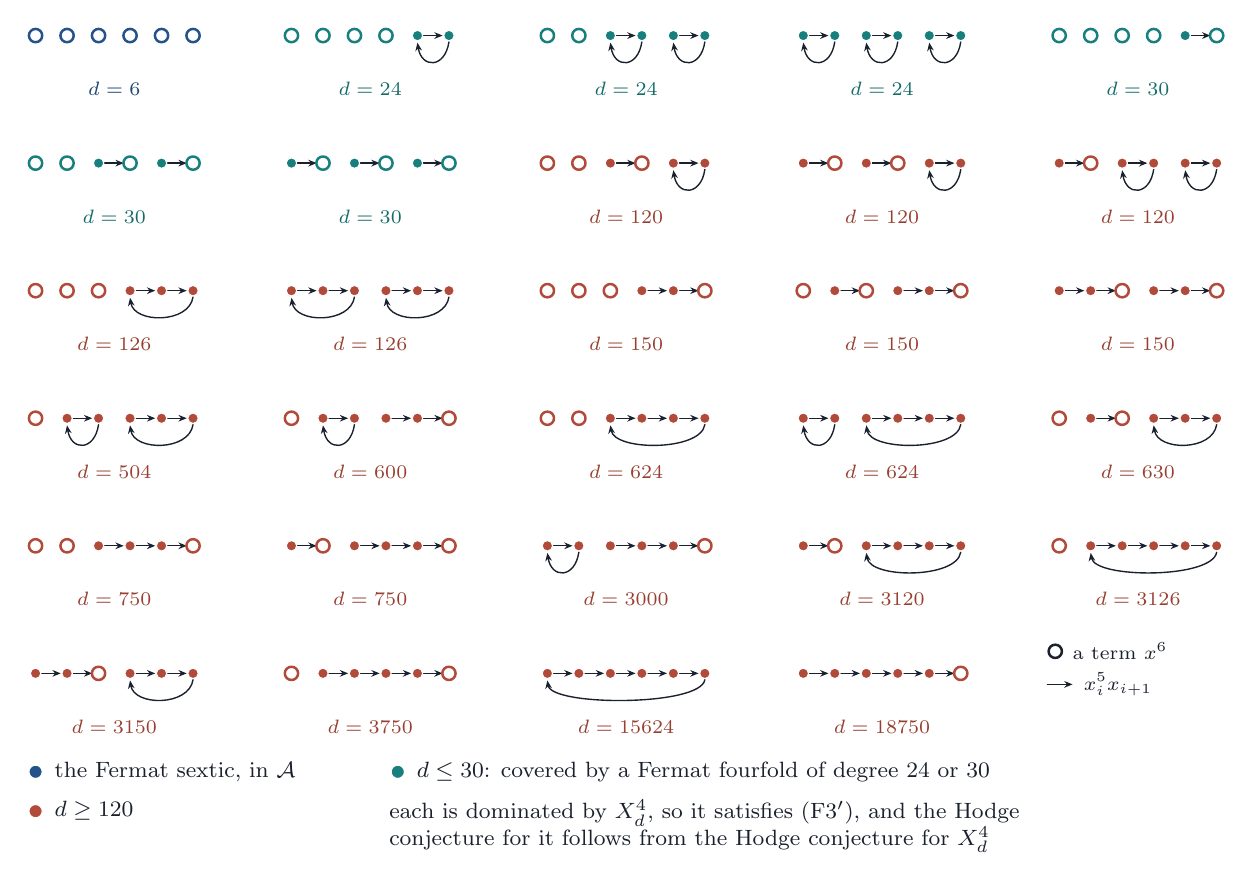
\begin{tikzpicture}[x=1cm,y=1cm,line join=round,line cap=round,
  font=\small,text=PInk,lbl/.style={inner sep=1pt}]
  \path[fill=white,draw=PBlue,line width=0.90pt] (0.3500,0.0000) circle (2.40pt);
  \path[fill=white,draw=PBlue,line width=0.90pt] (0.7500,0.0000) circle (2.40pt);
  \path[fill=white,draw=PBlue,line width=0.90pt] (1.1500,0.0000) circle (2.40pt);
  \path[fill=white,draw=PBlue,line width=0.90pt] (1.5500,0.0000) circle (2.40pt);
  \path[fill=white,draw=PBlue,line width=0.90pt] (1.9500,0.0000) circle (2.40pt);
  \path[fill=white,draw=PBlue,line width=0.90pt] (2.3500,0.0000) circle (2.40pt);
  \path[fill=white,draw=PTeal,line width=0.90pt] (3.6000,0.0000) circle (2.40pt);
  \path[fill=white,draw=PTeal,line width=0.90pt] (4.0000,0.0000) circle (2.40pt);
  \path[fill=white,draw=PTeal,line width=0.90pt] (4.4000,0.0000) circle (2.40pt);
  \path[fill=white,draw=PTeal,line width=0.90pt] (4.8000,0.0000) circle (2.40pt);
  \draw[PInk,line width=0.5pt,-{Stealth[length=3.0pt,width=2.4pt]}] (5.2700,0.0000) -- (5.5200,0.0000);
  \draw[PInk,line width=0.5pt,-{Stealth[length=3.0pt,width=2.4pt]}] (5.6000,-0.0800) .. controls (5.5500,-0.4200) and (5.2500,-0.4200) .. (5.2000,-0.0900);
  \path[fill=PTeal,draw=white,line width=0.40pt] (5.2000,0.0000) circle (1.90pt);
  \path[fill=PTeal,draw=white,line width=0.40pt] (5.6000,0.0000) circle (1.90pt);
  \path[fill=white,draw=PTeal,line width=0.90pt] (6.8500,0.0000) circle (2.40pt);
  \path[fill=white,draw=PTeal,line width=0.90pt] (7.2500,0.0000) circle (2.40pt);
  \draw[PInk,line width=0.5pt,-{Stealth[length=3.0pt,width=2.4pt]}] (7.7200,0.0000) -- (7.9700,0.0000);
  \draw[PInk,line width=0.5pt,-{Stealth[length=3.0pt,width=2.4pt]}] (8.0500,-0.0800) .. controls (8.0000,-0.4200) and (7.7000,-0.4200) .. (7.6500,-0.0900);
  \path[fill=PTeal,draw=white,line width=0.40pt] (7.6500,0.0000) circle (1.90pt);
  \path[fill=PTeal,draw=white,line width=0.40pt] (8.0500,0.0000) circle (1.90pt);
  \draw[PInk,line width=0.5pt,-{Stealth[length=3.0pt,width=2.4pt]}] (8.5200,0.0000) -- (8.7700,0.0000);
  \draw[PInk,line width=0.5pt,-{Stealth[length=3.0pt,width=2.4pt]}] (8.8500,-0.0800) .. controls (8.8000,-0.4200) and (8.5000,-0.4200) .. (8.4500,-0.0900);
  \path[fill=PTeal,draw=white,line width=0.40pt] (8.4500,0.0000) circle (1.90pt);
  \path[fill=PTeal,draw=white,line width=0.40pt] (8.8500,0.0000) circle (1.90pt);
  \draw[PInk,line width=0.5pt,-{Stealth[length=3.0pt,width=2.4pt]}] (10.1700,0.0000) -- (10.4200,0.0000);
  \draw[PInk,line width=0.5pt,-{Stealth[length=3.0pt,width=2.4pt]}] (10.5000,-0.0800) .. controls (10.4500,-0.4200) and (10.1500,-0.4200) .. (10.1000,-0.0900);
  \path[fill=PTeal,draw=white,line width=0.40pt] (10.1000,0.0000) circle (1.90pt);
  \path[fill=PTeal,draw=white,line width=0.40pt] (10.5000,0.0000) circle (1.90pt);
  \draw[PInk,line width=0.5pt,-{Stealth[length=3.0pt,width=2.4pt]}] (10.9700,0.0000) -- (11.2200,0.0000);
  \draw[PInk,line width=0.5pt,-{Stealth[length=3.0pt,width=2.4pt]}] (11.3000,-0.0800) .. controls (11.2500,-0.4200) and (10.9500,-0.4200) .. (10.9000,-0.0900);
  \path[fill=PTeal,draw=white,line width=0.40pt] (10.9000,0.0000) circle (1.90pt);
  \path[fill=PTeal,draw=white,line width=0.40pt] (11.3000,0.0000) circle (1.90pt);
  \draw[PInk,line width=0.5pt,-{Stealth[length=3.0pt,width=2.4pt]}] (11.7700,0.0000) -- (12.0200,0.0000);
  \draw[PInk,line width=0.5pt,-{Stealth[length=3.0pt,width=2.4pt]}] (12.1000,-0.0800) .. controls (12.0500,-0.4200) and (11.7500,-0.4200) .. (11.7000,-0.0900);
  \path[fill=PTeal,draw=white,line width=0.40pt] (11.7000,0.0000) circle (1.90pt);
  \path[fill=PTeal,draw=white,line width=0.40pt] (12.1000,0.0000) circle (1.90pt);
  \path[fill=white,draw=PTeal,line width=0.90pt] (13.3500,0.0000) circle (2.40pt);
  \path[fill=white,draw=PTeal,line width=0.90pt] (13.7500,0.0000) circle (2.40pt);
  \path[fill=white,draw=PTeal,line width=0.90pt] (14.1500,0.0000) circle (2.40pt);
  \path[fill=white,draw=PTeal,line width=0.90pt] (14.5500,0.0000) circle (2.40pt);
  \draw[PInk,line width=0.5pt,-{Stealth[length=3.0pt,width=2.4pt]}] (15.0200,0.0000) -- (15.2700,0.0000);
  \path[fill=PTeal,draw=white,line width=0.40pt] (14.9500,0.0000) circle (1.90pt);
  \path[fill=white,draw=PTeal,line width=0.90pt] (15.3500,0.0000) circle (2.40pt);
  \path[fill=white,draw=PTeal,line width=0.90pt] (0.3500,-1.6200) circle (2.40pt);
  \path[fill=white,draw=PTeal,line width=0.90pt] (0.7500,-1.6200) circle (2.40pt);
  \draw[PInk,line width=0.5pt,-{Stealth[length=3.0pt,width=2.4pt]}] (1.2200,-1.6200) -- (1.4700,-1.6200);
  \path[fill=PTeal,draw=white,line width=0.40pt] (1.1500,-1.6200) circle (1.90pt);
  \path[fill=white,draw=PTeal,line width=0.90pt] (1.5500,-1.6200) circle (2.40pt);
  \draw[PInk,line width=0.5pt,-{Stealth[length=3.0pt,width=2.4pt]}] (2.0200,-1.6200) -- (2.2700,-1.6200);
  \path[fill=PTeal,draw=white,line width=0.40pt] (1.9500,-1.6200) circle (1.90pt);
  \path[fill=white,draw=PTeal,line width=0.90pt] (2.3500,-1.6200) circle (2.40pt);
  \draw[PInk,line width=0.5pt,-{Stealth[length=3.0pt,width=2.4pt]}] (3.6700,-1.6200) -- (3.9200,-1.6200);
  \path[fill=PTeal,draw=white,line width=0.40pt] (3.6000,-1.6200) circle (1.90pt);
  \path[fill=white,draw=PTeal,line width=0.90pt] (4.0000,-1.6200) circle (2.40pt);
  \draw[PInk,line width=0.5pt,-{Stealth[length=3.0pt,width=2.4pt]}] (4.4700,-1.6200) -- (4.7200,-1.6200);
  \path[fill=PTeal,draw=white,line width=0.40pt] (4.4000,-1.6200) circle (1.90pt);
  \path[fill=white,draw=PTeal,line width=0.90pt] (4.8000,-1.6200) circle (2.40pt);
  \draw[PInk,line width=0.5pt,-{Stealth[length=3.0pt,width=2.4pt]}] (5.2700,-1.6200) -- (5.5200,-1.6200);
  \path[fill=PTeal,draw=white,line width=0.40pt] (5.2000,-1.6200) circle (1.90pt);
  \path[fill=white,draw=PTeal,line width=0.90pt] (5.6000,-1.6200) circle (2.40pt);
  \path[fill=white,draw=PClay,line width=0.90pt] (6.8500,-1.6200) circle (2.40pt);
  \path[fill=white,draw=PClay,line width=0.90pt] (7.2500,-1.6200) circle (2.40pt);
  \draw[PInk,line width=0.5pt,-{Stealth[length=3.0pt,width=2.4pt]}] (7.7200,-1.6200) -- (7.9700,-1.6200);
  \path[fill=PClay,draw=white,line width=0.40pt] (7.6500,-1.6200) circle (1.90pt);
  \path[fill=white,draw=PClay,line width=0.90pt] (8.0500,-1.6200) circle (2.40pt);
  \draw[PInk,line width=0.5pt,-{Stealth[length=3.0pt,width=2.4pt]}] (8.5200,-1.6200) -- (8.7700,-1.6200);
  \draw[PInk,line width=0.5pt,-{Stealth[length=3.0pt,width=2.4pt]}] (8.8500,-1.7000) .. controls (8.8000,-2.0400) and (8.5000,-2.0400) .. (8.4500,-1.7100);
  \path[fill=PClay,draw=white,line width=0.40pt] (8.4500,-1.6200) circle (1.90pt);
  \path[fill=PClay,draw=white,line width=0.40pt] (8.8500,-1.6200) circle (1.90pt);
  \draw[PInk,line width=0.5pt,-{Stealth[length=3.0pt,width=2.4pt]}] (10.1700,-1.6200) -- (10.4200,-1.6200);
  \path[fill=PClay,draw=white,line width=0.40pt] (10.1000,-1.6200) circle (1.90pt);
  \path[fill=white,draw=PClay,line width=0.90pt] (10.5000,-1.6200) circle (2.40pt);
  \draw[PInk,line width=0.5pt,-{Stealth[length=3.0pt,width=2.4pt]}] (10.9700,-1.6200) -- (11.2200,-1.6200);
  \path[fill=PClay,draw=white,line width=0.40pt] (10.9000,-1.6200) circle (1.90pt);
  \path[fill=white,draw=PClay,line width=0.90pt] (11.3000,-1.6200) circle (2.40pt);
  \draw[PInk,line width=0.5pt,-{Stealth[length=3.0pt,width=2.4pt]}] (11.7700,-1.6200) -- (12.0200,-1.6200);
  \draw[PInk,line width=0.5pt,-{Stealth[length=3.0pt,width=2.4pt]}] (12.1000,-1.7000) .. controls (12.0500,-2.0400) and (11.7500,-2.0400) .. (11.7000,-1.7100);
  \path[fill=PClay,draw=white,line width=0.40pt] (11.7000,-1.6200) circle (1.90pt);
  \path[fill=PClay,draw=white,line width=0.40pt] (12.1000,-1.6200) circle (1.90pt);
  \draw[PInk,line width=0.5pt,-{Stealth[length=3.0pt,width=2.4pt]}] (13.4200,-1.6200) -- (13.6700,-1.6200);
  \path[fill=PClay,draw=white,line width=0.40pt] (13.3500,-1.6200) circle (1.90pt);
  \path[fill=white,draw=PClay,line width=0.90pt] (13.7500,-1.6200) circle (2.40pt);
  \draw[PInk,line width=0.5pt,-{Stealth[length=3.0pt,width=2.4pt]}] (14.2200,-1.6200) -- (14.4700,-1.6200);
  \draw[PInk,line width=0.5pt,-{Stealth[length=3.0pt,width=2.4pt]}] (14.5500,-1.7000) .. controls (14.5000,-2.0400) and (14.2000,-2.0400) .. (14.1500,-1.7100);
  \path[fill=PClay,draw=white,line width=0.40pt] (14.1500,-1.6200) circle (1.90pt);
  \path[fill=PClay,draw=white,line width=0.40pt] (14.5500,-1.6200) circle (1.90pt);
  \draw[PInk,line width=0.5pt,-{Stealth[length=3.0pt,width=2.4pt]}] (15.0200,-1.6200) -- (15.2700,-1.6200);
  \draw[PInk,line width=0.5pt,-{Stealth[length=3.0pt,width=2.4pt]}] (15.3500,-1.7000) .. controls (15.3000,-2.0400) and (15.0000,-2.0400) .. (14.9500,-1.7100);
  \path[fill=PClay,draw=white,line width=0.40pt] (14.9500,-1.6200) circle (1.90pt);
  \path[fill=PClay,draw=white,line width=0.40pt] (15.3500,-1.6200) circle (1.90pt);
  \path[fill=white,draw=PClay,line width=0.90pt] (0.3500,-3.2400) circle (2.40pt);
  \path[fill=white,draw=PClay,line width=0.90pt] (0.7500,-3.2400) circle (2.40pt);
  \path[fill=white,draw=PClay,line width=0.90pt] (1.1500,-3.2400) circle (2.40pt);
  \draw[PInk,line width=0.5pt,-{Stealth[length=3.0pt,width=2.4pt]}] (1.6200,-3.2400) -- (1.8700,-3.2400);
  \draw[PInk,line width=0.5pt,-{Stealth[length=3.0pt,width=2.4pt]}] (2.0200,-3.2400) -- (2.2700,-3.2400);
  \draw[PInk,line width=0.5pt,-{Stealth[length=3.0pt,width=2.4pt]}] (2.3500,-3.3200) .. controls (2.3000,-3.6600) and (1.6000,-3.6600) .. (1.5500,-3.3300);
  \path[fill=PClay,draw=white,line width=0.40pt] (1.5500,-3.2400) circle (1.90pt);
  \path[fill=PClay,draw=white,line width=0.40pt] (1.9500,-3.2400) circle (1.90pt);
  \path[fill=PClay,draw=white,line width=0.40pt] (2.3500,-3.2400) circle (1.90pt);
  \draw[PInk,line width=0.5pt,-{Stealth[length=3.0pt,width=2.4pt]}] (3.6700,-3.2400) -- (3.9200,-3.2400);
  \draw[PInk,line width=0.5pt,-{Stealth[length=3.0pt,width=2.4pt]}] (4.0700,-3.2400) -- (4.3200,-3.2400);
  \draw[PInk,line width=0.5pt,-{Stealth[length=3.0pt,width=2.4pt]}] (4.4000,-3.3200) .. controls (4.3500,-3.6600) and (3.6500,-3.6600) .. (3.6000,-3.3300);
  \path[fill=PClay,draw=white,line width=0.40pt] (3.6000,-3.2400) circle (1.90pt);
  \path[fill=PClay,draw=white,line width=0.40pt] (4.0000,-3.2400) circle (1.90pt);
  \path[fill=PClay,draw=white,line width=0.40pt] (4.4000,-3.2400) circle (1.90pt);
  \draw[PInk,line width=0.5pt,-{Stealth[length=3.0pt,width=2.4pt]}] (4.8700,-3.2400) -- (5.1200,-3.2400);
  \draw[PInk,line width=0.5pt,-{Stealth[length=3.0pt,width=2.4pt]}] (5.2700,-3.2400) -- (5.5200,-3.2400);
  \draw[PInk,line width=0.5pt,-{Stealth[length=3.0pt,width=2.4pt]}] (5.6000,-3.3200) .. controls (5.5500,-3.6600) and (4.8500,-3.6600) .. (4.8000,-3.3300);
  \path[fill=PClay,draw=white,line width=0.40pt] (4.8000,-3.2400) circle (1.90pt);
  \path[fill=PClay,draw=white,line width=0.40pt] (5.2000,-3.2400) circle (1.90pt);
  \path[fill=PClay,draw=white,line width=0.40pt] (5.6000,-3.2400) circle (1.90pt);
  \path[fill=white,draw=PClay,line width=0.90pt] (6.8500,-3.2400) circle (2.40pt);
  \path[fill=white,draw=PClay,line width=0.90pt] (7.2500,-3.2400) circle (2.40pt);
  \path[fill=white,draw=PClay,line width=0.90pt] (7.6500,-3.2400) circle (2.40pt);
  \draw[PInk,line width=0.5pt,-{Stealth[length=3.0pt,width=2.4pt]}] (8.1200,-3.2400) -- (8.3700,-3.2400);
  \draw[PInk,line width=0.5pt,-{Stealth[length=3.0pt,width=2.4pt]}] (8.5200,-3.2400) -- (8.7700,-3.2400);
  \path[fill=PClay,draw=white,line width=0.40pt] (8.0500,-3.2400) circle (1.90pt);
  \path[fill=PClay,draw=white,line width=0.40pt] (8.4500,-3.2400) circle (1.90pt);
  \path[fill=white,draw=PClay,line width=0.90pt] (8.8500,-3.2400) circle (2.40pt);
  \path[fill=white,draw=PClay,line width=0.90pt] (10.1000,-3.2400) circle (2.40pt);
  \draw[PInk,line width=0.5pt,-{Stealth[length=3.0pt,width=2.4pt]}] (10.5700,-3.2400) -- (10.8200,-3.2400);
  \path[fill=PClay,draw=white,line width=0.40pt] (10.5000,-3.2400) circle (1.90pt);
  \path[fill=white,draw=PClay,line width=0.90pt] (10.9000,-3.2400) circle (2.40pt);
  \draw[PInk,line width=0.5pt,-{Stealth[length=3.0pt,width=2.4pt]}] (11.3700,-3.2400) -- (11.6200,-3.2400);
  \draw[PInk,line width=0.5pt,-{Stealth[length=3.0pt,width=2.4pt]}] (11.7700,-3.2400) -- (12.0200,-3.2400);
  \path[fill=PClay,draw=white,line width=0.40pt] (11.3000,-3.2400) circle (1.90pt);
  \path[fill=PClay,draw=white,line width=0.40pt] (11.7000,-3.2400) circle (1.90pt);
  \path[fill=white,draw=PClay,line width=0.90pt] (12.1000,-3.2400) circle (2.40pt);
  \draw[PInk,line width=0.5pt,-{Stealth[length=3.0pt,width=2.4pt]}] (13.4200,-3.2400) -- (13.6700,-3.2400);
  \draw[PInk,line width=0.5pt,-{Stealth[length=3.0pt,width=2.4pt]}] (13.8200,-3.2400) -- (14.0700,-3.2400);
  \path[fill=PClay,draw=white,line width=0.40pt] (13.3500,-3.2400) circle (1.90pt);
  \path[fill=PClay,draw=white,line width=0.40pt] (13.7500,-3.2400) circle (1.90pt);
  \path[fill=white,draw=PClay,line width=0.90pt] (14.1500,-3.2400) circle (2.40pt);
  \draw[PInk,line width=0.5pt,-{Stealth[length=3.0pt,width=2.4pt]}] (14.6200,-3.2400) -- (14.8700,-3.2400);
  \draw[PInk,line width=0.5pt,-{Stealth[length=3.0pt,width=2.4pt]}] (15.0200,-3.2400) -- (15.2700,-3.2400);
  \path[fill=PClay,draw=white,line width=0.40pt] (14.5500,-3.2400) circle (1.90pt);
  \path[fill=PClay,draw=white,line width=0.40pt] (14.9500,-3.2400) circle (1.90pt);
  \path[fill=white,draw=PClay,line width=0.90pt] (15.3500,-3.2400) circle (2.40pt);
  \path[fill=white,draw=PClay,line width=0.90pt] (0.3500,-4.8600) circle (2.40pt);
  \draw[PInk,line width=0.5pt,-{Stealth[length=3.0pt,width=2.4pt]}] (0.8200,-4.8600) -- (1.0700,-4.8600);
  \draw[PInk,line width=0.5pt,-{Stealth[length=3.0pt,width=2.4pt]}] (1.1500,-4.9400) .. controls (1.1000,-5.2800) and (0.8000,-5.2800) .. (0.7500,-4.9500);
  \path[fill=PClay,draw=white,line width=0.40pt] (0.7500,-4.8600) circle (1.90pt);
  \path[fill=PClay,draw=white,line width=0.40pt] (1.1500,-4.8600) circle (1.90pt);
  \draw[PInk,line width=0.5pt,-{Stealth[length=3.0pt,width=2.4pt]}] (1.6200,-4.8600) -- (1.8700,-4.8600);
  \draw[PInk,line width=0.5pt,-{Stealth[length=3.0pt,width=2.4pt]}] (2.0200,-4.8600) -- (2.2700,-4.8600);
  \draw[PInk,line width=0.5pt,-{Stealth[length=3.0pt,width=2.4pt]}] (2.3500,-4.9400) .. controls (2.3000,-5.2800) and (1.6000,-5.2800) .. (1.5500,-4.9500);
  \path[fill=PClay,draw=white,line width=0.40pt] (1.5500,-4.8600) circle (1.90pt);
  \path[fill=PClay,draw=white,line width=0.40pt] (1.9500,-4.8600) circle (1.90pt);
  \path[fill=PClay,draw=white,line width=0.40pt] (2.3500,-4.8600) circle (1.90pt);
  \path[fill=white,draw=PClay,line width=0.90pt] (3.6000,-4.8600) circle (2.40pt);
  \draw[PInk,line width=0.5pt,-{Stealth[length=3.0pt,width=2.4pt]}] (4.0700,-4.8600) -- (4.3200,-4.8600);
  \draw[PInk,line width=0.5pt,-{Stealth[length=3.0pt,width=2.4pt]}] (4.4000,-4.9400) .. controls (4.3500,-5.2800) and (4.0500,-5.2800) .. (4.0000,-4.9500);
  \path[fill=PClay,draw=white,line width=0.40pt] (4.0000,-4.8600) circle (1.90pt);
  \path[fill=PClay,draw=white,line width=0.40pt] (4.4000,-4.8600) circle (1.90pt);
  \draw[PInk,line width=0.5pt,-{Stealth[length=3.0pt,width=2.4pt]}] (4.8700,-4.8600) -- (5.1200,-4.8600);
  \draw[PInk,line width=0.5pt,-{Stealth[length=3.0pt,width=2.4pt]}] (5.2700,-4.8600) -- (5.5200,-4.8600);
  \path[fill=PClay,draw=white,line width=0.40pt] (4.8000,-4.8600) circle (1.90pt);
  \path[fill=PClay,draw=white,line width=0.40pt] (5.2000,-4.8600) circle (1.90pt);
  \path[fill=white,draw=PClay,line width=0.90pt] (5.6000,-4.8600) circle (2.40pt);
  \path[fill=white,draw=PClay,line width=0.90pt] (6.8500,-4.8600) circle (2.40pt);
  \path[fill=white,draw=PClay,line width=0.90pt] (7.2500,-4.8600) circle (2.40pt);
  \draw[PInk,line width=0.5pt,-{Stealth[length=3.0pt,width=2.4pt]}] (7.7200,-4.8600) -- (7.9700,-4.8600);
  \draw[PInk,line width=0.5pt,-{Stealth[length=3.0pt,width=2.4pt]}] (8.1200,-4.8600) -- (8.3700,-4.8600);
  \draw[PInk,line width=0.5pt,-{Stealth[length=3.0pt,width=2.4pt]}] (8.5200,-4.8600) -- (8.7700,-4.8600);
  \draw[PInk,line width=0.5pt,-{Stealth[length=3.0pt,width=2.4pt]}] (8.8500,-4.9400) .. controls (8.8000,-5.2800) and (7.7000,-5.2800) .. (7.6500,-4.9500);
  \path[fill=PClay,draw=white,line width=0.40pt] (7.6500,-4.8600) circle (1.90pt);
  \path[fill=PClay,draw=white,line width=0.40pt] (8.0500,-4.8600) circle (1.90pt);
  \path[fill=PClay,draw=white,line width=0.40pt] (8.4500,-4.8600) circle (1.90pt);
  \path[fill=PClay,draw=white,line width=0.40pt] (8.8500,-4.8600) circle (1.90pt);
  \draw[PInk,line width=0.5pt,-{Stealth[length=3.0pt,width=2.4pt]}] (10.1700,-4.8600) -- (10.4200,-4.8600);
  \draw[PInk,line width=0.5pt,-{Stealth[length=3.0pt,width=2.4pt]}] (10.5000,-4.9400) .. controls (10.4500,-5.2800) and (10.1500,-5.2800) .. (10.1000,-4.9500);
  \path[fill=PClay,draw=white,line width=0.40pt] (10.1000,-4.8600) circle (1.90pt);
  \path[fill=PClay,draw=white,line width=0.40pt] (10.5000,-4.8600) circle (1.90pt);
  \draw[PInk,line width=0.5pt,-{Stealth[length=3.0pt,width=2.4pt]}] (10.9700,-4.8600) -- (11.2200,-4.8600);
  \draw[PInk,line width=0.5pt,-{Stealth[length=3.0pt,width=2.4pt]}] (11.3700,-4.8600) -- (11.6200,-4.8600);
  \draw[PInk,line width=0.5pt,-{Stealth[length=3.0pt,width=2.4pt]}] (11.7700,-4.8600) -- (12.0200,-4.8600);
  \draw[PInk,line width=0.5pt,-{Stealth[length=3.0pt,width=2.4pt]}] (12.1000,-4.9400) .. controls (12.0500,-5.2800) and (10.9500,-5.2800) .. (10.9000,-4.9500);
  \path[fill=PClay,draw=white,line width=0.40pt] (10.9000,-4.8600) circle (1.90pt);
  \path[fill=PClay,draw=white,line width=0.40pt] (11.3000,-4.8600) circle (1.90pt);
  \path[fill=PClay,draw=white,line width=0.40pt] (11.7000,-4.8600) circle (1.90pt);
  \path[fill=PClay,draw=white,line width=0.40pt] (12.1000,-4.8600) circle (1.90pt);
  \path[fill=white,draw=PClay,line width=0.90pt] (13.3500,-4.8600) circle (2.40pt);
  \draw[PInk,line width=0.5pt,-{Stealth[length=3.0pt,width=2.4pt]}] (13.8200,-4.8600) -- (14.0700,-4.8600);
  \path[fill=PClay,draw=white,line width=0.40pt] (13.7500,-4.8600) circle (1.90pt);
  \path[fill=white,draw=PClay,line width=0.90pt] (14.1500,-4.8600) circle (2.40pt);
  \draw[PInk,line width=0.5pt,-{Stealth[length=3.0pt,width=2.4pt]}] (14.6200,-4.8600) -- (14.8700,-4.8600);
  \draw[PInk,line width=0.5pt,-{Stealth[length=3.0pt,width=2.4pt]}] (15.0200,-4.8600) -- (15.2700,-4.8600);
  \draw[PInk,line width=0.5pt,-{Stealth[length=3.0pt,width=2.4pt]}] (15.3500,-4.9400) .. controls (15.3000,-5.2800) and (14.6000,-5.2800) .. (14.5500,-4.9500);
  \path[fill=PClay,draw=white,line width=0.40pt] (14.5500,-4.8600) circle (1.90pt);
  \path[fill=PClay,draw=white,line width=0.40pt] (14.9500,-4.8600) circle (1.90pt);
  \path[fill=PClay,draw=white,line width=0.40pt] (15.3500,-4.8600) circle (1.90pt);
  \path[fill=white,draw=PClay,line width=0.90pt] (0.3500,-6.4800) circle (2.40pt);
  \path[fill=white,draw=PClay,line width=0.90pt] (0.7500,-6.4800) circle (2.40pt);
  \draw[PInk,line width=0.5pt,-{Stealth[length=3.0pt,width=2.4pt]}] (1.2200,-6.4800) -- (1.4700,-6.4800);
  \draw[PInk,line width=0.5pt,-{Stealth[length=3.0pt,width=2.4pt]}] (1.6200,-6.4800) -- (1.8700,-6.4800);
  \draw[PInk,line width=0.5pt,-{Stealth[length=3.0pt,width=2.4pt]}] (2.0200,-6.4800) -- (2.2700,-6.4800);
  \path[fill=PClay,draw=white,line width=0.40pt] (1.1500,-6.4800) circle (1.90pt);
  \path[fill=PClay,draw=white,line width=0.40pt] (1.5500,-6.4800) circle (1.90pt);
  \path[fill=PClay,draw=white,line width=0.40pt] (1.9500,-6.4800) circle (1.90pt);
  \path[fill=white,draw=PClay,line width=0.90pt] (2.3500,-6.4800) circle (2.40pt);
  \draw[PInk,line width=0.5pt,-{Stealth[length=3.0pt,width=2.4pt]}] (3.6700,-6.4800) -- (3.9200,-6.4800);
  \path[fill=PClay,draw=white,line width=0.40pt] (3.6000,-6.4800) circle (1.90pt);
  \path[fill=white,draw=PClay,line width=0.90pt] (4.0000,-6.4800) circle (2.40pt);
  \draw[PInk,line width=0.5pt,-{Stealth[length=3.0pt,width=2.4pt]}] (4.4700,-6.4800) -- (4.7200,-6.4800);
  \draw[PInk,line width=0.5pt,-{Stealth[length=3.0pt,width=2.4pt]}] (4.8700,-6.4800) -- (5.1200,-6.4800);
  \draw[PInk,line width=0.5pt,-{Stealth[length=3.0pt,width=2.4pt]}] (5.2700,-6.4800) -- (5.5200,-6.4800);
  \path[fill=PClay,draw=white,line width=0.40pt] (4.4000,-6.4800) circle (1.90pt);
  \path[fill=PClay,draw=white,line width=0.40pt] (4.8000,-6.4800) circle (1.90pt);
  \path[fill=PClay,draw=white,line width=0.40pt] (5.2000,-6.4800) circle (1.90pt);
  \path[fill=white,draw=PClay,line width=0.90pt] (5.6000,-6.4800) circle (2.40pt);
  \draw[PInk,line width=0.5pt,-{Stealth[length=3.0pt,width=2.4pt]}] (6.9200,-6.4800) -- (7.1700,-6.4800);
  \draw[PInk,line width=0.5pt,-{Stealth[length=3.0pt,width=2.4pt]}] (7.2500,-6.5600) .. controls (7.2000,-6.9000) and (6.9000,-6.9000) .. (6.8500,-6.5700);
  \path[fill=PClay,draw=white,line width=0.40pt] (6.8500,-6.4800) circle (1.90pt);
  \path[fill=PClay,draw=white,line width=0.40pt] (7.2500,-6.4800) circle (1.90pt);
  \draw[PInk,line width=0.5pt,-{Stealth[length=3.0pt,width=2.4pt]}] (7.7200,-6.4800) -- (7.9700,-6.4800);
  \draw[PInk,line width=0.5pt,-{Stealth[length=3.0pt,width=2.4pt]}] (8.1200,-6.4800) -- (8.3700,-6.4800);
  \draw[PInk,line width=0.5pt,-{Stealth[length=3.0pt,width=2.4pt]}] (8.5200,-6.4800) -- (8.7700,-6.4800);
  \path[fill=PClay,draw=white,line width=0.40pt] (7.6500,-6.4800) circle (1.90pt);
  \path[fill=PClay,draw=white,line width=0.40pt] (8.0500,-6.4800) circle (1.90pt);
  \path[fill=PClay,draw=white,line width=0.40pt] (8.4500,-6.4800) circle (1.90pt);
  \path[fill=white,draw=PClay,line width=0.90pt] (8.8500,-6.4800) circle (2.40pt);
  \draw[PInk,line width=0.5pt,-{Stealth[length=3.0pt,width=2.4pt]}] (10.1700,-6.4800) -- (10.4200,-6.4800);
  \path[fill=PClay,draw=white,line width=0.40pt] (10.1000,-6.4800) circle (1.90pt);
  \path[fill=white,draw=PClay,line width=0.90pt] (10.5000,-6.4800) circle (2.40pt);
  \draw[PInk,line width=0.5pt,-{Stealth[length=3.0pt,width=2.4pt]}] (10.9700,-6.4800) -- (11.2200,-6.4800);
  \draw[PInk,line width=0.5pt,-{Stealth[length=3.0pt,width=2.4pt]}] (11.3700,-6.4800) -- (11.6200,-6.4800);
  \draw[PInk,line width=0.5pt,-{Stealth[length=3.0pt,width=2.4pt]}] (11.7700,-6.4800) -- (12.0200,-6.4800);
  \draw[PInk,line width=0.5pt,-{Stealth[length=3.0pt,width=2.4pt]}] (12.1000,-6.5600) .. controls (12.0500,-6.9000) and (10.9500,-6.9000) .. (10.9000,-6.5700);
  \path[fill=PClay,draw=white,line width=0.40pt] (10.9000,-6.4800) circle (1.90pt);
  \path[fill=PClay,draw=white,line width=0.40pt] (11.3000,-6.4800) circle (1.90pt);
  \path[fill=PClay,draw=white,line width=0.40pt] (11.7000,-6.4800) circle (1.90pt);
  \path[fill=PClay,draw=white,line width=0.40pt] (12.1000,-6.4800) circle (1.90pt);
  \path[fill=white,draw=PClay,line width=0.90pt] (13.3500,-6.4800) circle (2.40pt);
  \draw[PInk,line width=0.5pt,-{Stealth[length=3.0pt,width=2.4pt]}] (13.8200,-6.4800) -- (14.0700,-6.4800);
  \draw[PInk,line width=0.5pt,-{Stealth[length=3.0pt,width=2.4pt]}] (14.2200,-6.4800) -- (14.4700,-6.4800);
  \draw[PInk,line width=0.5pt,-{Stealth[length=3.0pt,width=2.4pt]}] (14.6200,-6.4800) -- (14.8700,-6.4800);
  \draw[PInk,line width=0.5pt,-{Stealth[length=3.0pt,width=2.4pt]}] (15.0200,-6.4800) -- (15.2700,-6.4800);
  \draw[PInk,line width=0.5pt,-{Stealth[length=3.0pt,width=2.4pt]}] (15.3500,-6.5600) .. controls (15.3000,-6.9000) and (13.8000,-6.9000) .. (13.7500,-6.5700);
  \path[fill=PClay,draw=white,line width=0.40pt] (13.7500,-6.4800) circle (1.90pt);
  \path[fill=PClay,draw=white,line width=0.40pt] (14.1500,-6.4800) circle (1.90pt);
  \path[fill=PClay,draw=white,line width=0.40pt] (14.5500,-6.4800) circle (1.90pt);
  \path[fill=PClay,draw=white,line width=0.40pt] (14.9500,-6.4800) circle (1.90pt);
  \path[fill=PClay,draw=white,line width=0.40pt] (15.3500,-6.4800) circle (1.90pt);
  \draw[PInk,line width=0.5pt,-{Stealth[length=3.0pt,width=2.4pt]}] (0.4200,-8.1000) -- (0.6700,-8.1000);
  \draw[PInk,line width=0.5pt,-{Stealth[length=3.0pt,width=2.4pt]}] (0.8200,-8.1000) -- (1.0700,-8.1000);
  \path[fill=PClay,draw=white,line width=0.40pt] (0.3500,-8.1000) circle (1.90pt);
  \path[fill=PClay,draw=white,line width=0.40pt] (0.7500,-8.1000) circle (1.90pt);
  \path[fill=white,draw=PClay,line width=0.90pt] (1.1500,-8.1000) circle (2.40pt);
  \draw[PInk,line width=0.5pt,-{Stealth[length=3.0pt,width=2.4pt]}] (1.6200,-8.1000) -- (1.8700,-8.1000);
  \draw[PInk,line width=0.5pt,-{Stealth[length=3.0pt,width=2.4pt]}] (2.0200,-8.1000) -- (2.2700,-8.1000);
  \draw[PInk,line width=0.5pt,-{Stealth[length=3.0pt,width=2.4pt]}] (2.3500,-8.1800) .. controls (2.3000,-8.5200) and (1.6000,-8.5200) .. (1.5500,-8.1900);
  \path[fill=PClay,draw=white,line width=0.40pt] (1.5500,-8.1000) circle (1.90pt);
  \path[fill=PClay,draw=white,line width=0.40pt] (1.9500,-8.1000) circle (1.90pt);
  \path[fill=PClay,draw=white,line width=0.40pt] (2.3500,-8.1000) circle (1.90pt);
  \path[fill=white,draw=PClay,line width=0.90pt] (3.6000,-8.1000) circle (2.40pt);
  \draw[PInk,line width=0.5pt,-{Stealth[length=3.0pt,width=2.4pt]}] (4.0700,-8.1000) -- (4.3200,-8.1000);
  \draw[PInk,line width=0.5pt,-{Stealth[length=3.0pt,width=2.4pt]}] (4.4700,-8.1000) -- (4.7200,-8.1000);
  \draw[PInk,line width=0.5pt,-{Stealth[length=3.0pt,width=2.4pt]}] (4.8700,-8.1000) -- (5.1200,-8.1000);
  \draw[PInk,line width=0.5pt,-{Stealth[length=3.0pt,width=2.4pt]}] (5.2700,-8.1000) -- (5.5200,-8.1000);
  \path[fill=PClay,draw=white,line width=0.40pt] (4.0000,-8.1000) circle (1.90pt);
  \path[fill=PClay,draw=white,line width=0.40pt] (4.4000,-8.1000) circle (1.90pt);
  \path[fill=PClay,draw=white,line width=0.40pt] (4.8000,-8.1000) circle (1.90pt);
  \path[fill=PClay,draw=white,line width=0.40pt] (5.2000,-8.1000) circle (1.90pt);
  \path[fill=white,draw=PClay,line width=0.90pt] (5.6000,-8.1000) circle (2.40pt);
  \draw[PInk,line width=0.5pt,-{Stealth[length=3.0pt,width=2.4pt]}] (6.9200,-8.1000) -- (7.1700,-8.1000);
  \draw[PInk,line width=0.5pt,-{Stealth[length=3.0pt,width=2.4pt]}] (7.3200,-8.1000) -- (7.5700,-8.1000);
  \draw[PInk,line width=0.5pt,-{Stealth[length=3.0pt,width=2.4pt]}] (7.7200,-8.1000) -- (7.9700,-8.1000);
  \draw[PInk,line width=0.5pt,-{Stealth[length=3.0pt,width=2.4pt]}] (8.1200,-8.1000) -- (8.3700,-8.1000);
  \draw[PInk,line width=0.5pt,-{Stealth[length=3.0pt,width=2.4pt]}] (8.5200,-8.1000) -- (8.7700,-8.1000);
  \draw[PInk,line width=0.5pt,-{Stealth[length=3.0pt,width=2.4pt]}] (8.8500,-8.1800) .. controls (8.8000,-8.5200) and (6.9000,-8.5200) .. (6.8500,-8.1900);
  \path[fill=PClay,draw=white,line width=0.40pt] (6.8500,-8.1000) circle (1.90pt);
  \path[fill=PClay,draw=white,line width=0.40pt] (7.2500,-8.1000) circle (1.90pt);
  \path[fill=PClay,draw=white,line width=0.40pt] (7.6500,-8.1000) circle (1.90pt);
  \path[fill=PClay,draw=white,line width=0.40pt] (8.0500,-8.1000) circle (1.90pt);
  \path[fill=PClay,draw=white,line width=0.40pt] (8.4500,-8.1000) circle (1.90pt);
  \path[fill=PClay,draw=white,line width=0.40pt] (8.8500,-8.1000) circle (1.90pt);
  \draw[PInk,line width=0.5pt,-{Stealth[length=3.0pt,width=2.4pt]}] (10.1700,-8.1000) -- (10.4200,-8.1000);
  \draw[PInk,line width=0.5pt,-{Stealth[length=3.0pt,width=2.4pt]}] (10.5700,-8.1000) -- (10.8200,-8.1000);
  \draw[PInk,line width=0.5pt,-{Stealth[length=3.0pt,width=2.4pt]}] (10.9700,-8.1000) -- (11.2200,-8.1000);
  \draw[PInk,line width=0.5pt,-{Stealth[length=3.0pt,width=2.4pt]}] (11.3700,-8.1000) -- (11.6200,-8.1000);
  \draw[PInk,line width=0.5pt,-{Stealth[length=3.0pt,width=2.4pt]}] (11.7700,-8.1000) -- (12.0200,-8.1000);
  \path[fill=PClay,draw=white,line width=0.40pt] (10.1000,-8.1000) circle (1.90pt);
  \path[fill=PClay,draw=white,line width=0.40pt] (10.5000,-8.1000) circle (1.90pt);
  \path[fill=PClay,draw=white,line width=0.40pt] (10.9000,-8.1000) circle (1.90pt);
  \path[fill=PClay,draw=white,line width=0.40pt] (11.3000,-8.1000) circle (1.90pt);
  \path[fill=PClay,draw=white,line width=0.40pt] (11.7000,-8.1000) circle (1.90pt);
  \path[fill=white,draw=PClay,line width=0.90pt] (12.1000,-8.1000) circle (2.40pt);
  \path[fill=white,draw=PInk,line width=0.90pt] (13.3000,-7.8200) circle (2.40pt);
  \draw[PInk,line width=0.5pt,-{Stealth[length=3.0pt,width=2.4pt]}] (13.2000,-8.2400) -- (13.5200,-8.2400);
  \path[fill=PBlue,draw=white,line width=0.40pt] (0.3500,-9.3500) circle (2.40pt);
  \path[fill=PTeal,draw=white,line width=0.40pt] (4.9500,-9.3500) circle (2.40pt);
  \path[fill=PClay,draw=white,line width=0.40pt] (0.3500,-9.8500) circle (2.40pt);
  \node[lbl,anchor=north,text=PBlue!85!black,font=\scriptsize] at (1.3500,-0.5500) {$d=6$};
  \node[lbl,anchor=north,text=PTeal!85!black,font=\scriptsize] at (4.6000,-0.5500) {$d=24$};
  \node[lbl,anchor=north,text=PTeal!85!black,font=\scriptsize] at (7.8500,-0.5500) {$d=24$};
  \node[lbl,anchor=north,text=PTeal!85!black,font=\scriptsize] at (11.1000,-0.5500) {$d=24$};
  \node[lbl,anchor=north,text=PTeal!85!black,font=\scriptsize] at (14.3500,-0.5500) {$d=30$};
  \node[lbl,anchor=north,text=PTeal!85!black,font=\scriptsize] at (1.3500,-2.1700) {$d=30$};
  \node[lbl,anchor=north,text=PTeal!85!black,font=\scriptsize] at (4.6000,-2.1700) {$d=30$};
  \node[lbl,anchor=north,text=PClay!85!black,font=\scriptsize] at (7.8500,-2.1700) {$d=120$};
  \node[lbl,anchor=north,text=PClay!85!black,font=\scriptsize] at (11.1000,-2.1700) {$d=120$};
  \node[lbl,anchor=north,text=PClay!85!black,font=\scriptsize] at (14.3500,-2.1700) {$d=120$};
  \node[lbl,anchor=north,text=PClay!85!black,font=\scriptsize] at (1.3500,-3.7900) {$d=126$};
  \node[lbl,anchor=north,text=PClay!85!black,font=\scriptsize] at (4.6000,-3.7900) {$d=126$};
  \node[lbl,anchor=north,text=PClay!85!black,font=\scriptsize] at (7.8500,-3.7900) {$d=150$};
  \node[lbl,anchor=north,text=PClay!85!black,font=\scriptsize] at (11.1000,-3.7900) {$d=150$};
  \node[lbl,anchor=north,text=PClay!85!black,font=\scriptsize] at (14.3500,-3.7900) {$d=150$};
  \node[lbl,anchor=north,text=PClay!85!black,font=\scriptsize] at (1.3500,-5.4100) {$d=504$};
  \node[lbl,anchor=north,text=PClay!85!black,font=\scriptsize] at (4.6000,-5.4100) {$d=600$};
  \node[lbl,anchor=north,text=PClay!85!black,font=\scriptsize] at (7.8500,-5.4100) {$d=624$};
  \node[lbl,anchor=north,text=PClay!85!black,font=\scriptsize] at (11.1000,-5.4100) {$d=624$};
  \node[lbl,anchor=north,text=PClay!85!black,font=\scriptsize] at (14.3500,-5.4100) {$d=630$};
  \node[lbl,anchor=north,text=PClay!85!black,font=\scriptsize] at (1.3500,-7.0300) {$d=750$};
  \node[lbl,anchor=north,text=PClay!85!black,font=\scriptsize] at (4.6000,-7.0300) {$d=750$};
  \node[lbl,anchor=north,text=PClay!85!black,font=\scriptsize] at (7.8500,-7.0300) {$d=3000$};
  \node[lbl,anchor=north,text=PClay!85!black,font=\scriptsize] at (11.1000,-7.0300) {$d=3120$};
  \node[lbl,anchor=north,text=PClay!85!black,font=\scriptsize] at (14.3500,-7.0300) {$d=3126$};
  \node[lbl,anchor=north,text=PClay!85!black,font=\scriptsize] at (1.3500,-8.6500) {$d=3150$};
  \node[lbl,anchor=north,text=PClay!85!black,font=\scriptsize] at (4.6000,-8.6500) {$d=3750$};
  \node[lbl,anchor=north,text=PClay!85!black,font=\scriptsize] at (7.8500,-8.6500) {$d=15624$};
  \node[lbl,anchor=north,text=PClay!85!black,font=\scriptsize] at (11.1000,-8.6500) {$d=18750$};
  \node[lbl,anchor=west,text=PInk,font=\scriptsize] at (13.4800,-7.8200) {a term $x^{6}$};
  \node[lbl,anchor=west,text=PInk,font=\scriptsize] at (13.6200,-8.2400) {$x_{i}^{5}x_{i+1}$};
  \node[lbl,anchor=west,text=PInk,font=\footnotesize] at (0.5500,-9.3500) {the Fermat sextic, in $\mathcal{A}$};
  \node[lbl,anchor=west,text=PInk,font=\footnotesize] at (5.1500,-9.3500) {$d\le30$: covered by a Fermat fourfold of degree $24$ or $30$};
  \node[lbl,anchor=west,text=PInk,font=\footnotesize] at (0.5500,-9.8500) {$d\ge120$};
  \node[lbl,anchor=west,text=PInk,font=\footnotesize,align=left] at (4.8000,-10.0456) {each is dominated by $X^{4}_{d}$, so it satisfies (F3$'$), and the Hodge\\conjecture for it follows from the Hodge conjecture for $X^{4}_{d}$};
\end{tikzpicture}
\end{document}
